% mnras_template.tex
%
% LaTeX template for creating an MNRAS paper
%
% v3.0 released 14 May 2015
% (version numbers match those of mnras.cls)
%
% Copyright (C) Royal Astronomical Society 2015
% Authors:
% Keith T. Smith (Royal Astronomical Society)

% Change log
%
% v3.0 May 2015
%    Renamed to match the new package name
%    Version number matches mnras.cls
%    A few minor tweaks to wording
% v1.0 September 2013
%    Beta testing only - never publicly released
%    First version: a simple (ish) template for creating an MNRAS paper

%%%%%%%%%%%%%%%%%%%%%%%%%%%%%%%%%%%%%%%%%%%%%%%%%%
% Basic setup. Most papers should leave these options alone.
\documentclass[a4paper,fleqn,usenatbib]{mnras}

% MNRAS is set in Times font. If you don't have this installed (most LaTeX
% installations will be fine) or prefer the old Computer Modern fonts, comment
% out the following line
%\usepackage{newtxtext,newtxmath}
% Depending on your LaTeX fonts installation, you might get better results with one of these:
%\usepackage{mathptmx}
%\usepackage{txfonts}

% Use vector fonts, so it zooms properly in on-screen viewing software
% Don't change these lines unless you know what you are doing
\usepackage[T1]{fontenc}
\usepackage{ae,aecompl}



%%%%% AUTHORS - PLACE YOUR OWN PACKAGES HERE %%%%%

% Only include extra packages if you really need them. Common packages are:
\usepackage[linesnumbered,ruled]{algorithm2e}
\usepackage[]{algorithm2e}
\usepackage{graphicx}	% Including figure files
\usepackage{amsmath}	% Advanced maths commands
\usepackage{amssymb}	% Extra maths symbols
\usepackage[latin1]{inputenc}
\usepackage{tikz}
\usetikzlibrary{shapes,arrows}


%-- Colours
\definecolor{mustard}{rgb}{1.0, 0.86, 0.35}
\definecolor{cyan(process)}{rgb}{0.0, 0.72, 0.92}
\definecolor{ochre}{rgb}{0.8, 0.47, 0.13}
\definecolor{linesOne}{rgb}{0, 0.4470, 0.7410}
\definecolor{linesTwo}{rgb}{0.8500, 0.3250, 0.0980}
\definecolor{linesThree}{rgb}{0.9290, 0.6940, 0.1250}
\definecolor{linesFour}{rgb}{0.4940, 0.1840, 0.5560}
\definecolor{linesFive}{rgb}{0.4660, 0.6740, 0.1880}

\newcommand{\lone}[1]{\textbf{\textcolor{linesOne}{#1}}}
\newcommand{\ltwo}[1]{\textbf{\textcolor{linesTwo}{#1}}}
\newcommand{\lthree}[1]{\textbf{\textcolor{linesThree}{#1}}}
\newcommand{\lfour}[1]{\textbf{\textcolor{linesFour}{#1}}}


%-- Editor commands
\newcommand{\floor}[1]{\textbf{\textcolor{ochre}{#1}}}
\newcommand{\selma}[1]{\textbf{\textcolor{cyan(process)}{#1}}}
\newcommand{\ilya}[1]{\textbf{\textcolor{magenta}{#1}}}
\newcommand{\stephen}[1]{\textbf{\textcolor{linesFive}{#1}}}
\newcommand{\todo}[1]{{\color{red}#1}}
\newcommand\Fiducial{\texttt{Fiducial }}
\newcommand\CompasAlpha{\texttt{COMPAS$_\alpha$}}
\newcommand\rate{\mathcal{R}}





%-- Constants
%\newcommand\hubbleTimeGyrs{14.6353}
\newcommand\hubbleTimeGyrs{14.03}

\newcommand\ratezero{X}
\newcommand\errorratezero{x}


\newcommand{\SpeedUpALLone}{25$\times$}
\newcommand{\SpeedUpALLoneTenmillion}{33$\times$}
\newcommand\HitsALLMCone{7734}
\newcommand\HitsALLAISone{261435}
\newcommand{\fractionMoreHitsALLone}{34$\times$}

\newcommand{\SpeedUpALLtwo}{28$\times$}
\newcommand{\SpeedUpALLtwoTenmillion}{41$\times$}
\newcommand\HitsALLMCtwo{6929}
\newcommand\HitsALLAIStwo{292746}
\newcommand{\fractionMoreHitsALLtwo}{42$\times$}

\newcommand{\SpeedUpBHNSone}{10$\times$}
\newcommand{\SpeedUpBHNSoneTenmillion}{55$\times$}
\newcommand\HitsBHNSMCone{1015}
\newcommand\HitsBHNSAISone{97817}
\newcommand{\fractionMoreHitsBHNSone}{96$\times$}
%\newcommand\MonteCarlo{9.169hrs}
%\newcommand\ExploratoryPhase{9.14hrs}
\newcommand{\SpeedUpBHNStwo}{16$\times$}
\newcommand{\SpeedUpBHNStwoTenmillion}{80$\times$}
\newcommand\HitsBHNSMCtwo{1345}
\newcommand\HitsBHNSAIStwo{194630}
\newcommand{\fractionMoreHitsBHNStwo}{145$\times$}

%%%%%%%%%%%%%%%%%%%%%%%%%%%%%%%%%%%%%%%%%%%%%%%%%%

%%%%% AUTHORS - PLACE YOUR OWN COMMANDS HERE %%%%%

% Please keep new commands to a minimum, and use \newcommand not \def to avoid
% overwriting existing commands. Example:
%\newcommand{\pcm}{\,cm$^{-2}$}	% per cm-squared

%%%%%%%%%%%%%%%%%%%%%%%%%%%%%%%%%%%%%%%%%%%%%%%%%%

%%%%%%%%%%%%%%%%%%% TITLE PAGE %%%%%%%%%%%%%%%%%%%

% Title of the paper, and the short title which is used in the headers.
% Keep the title short and informative.
\title[Black Hole - Neutron Star ]{On a Detailed Study of Black Hole-Neutron Star Mergers: \\ improving  population studies of rare events.}
% On a Detailed Study of Black Hole - Neutron Star Mergers: \\ speeding up inference studies of rare events
% A Detailed Study of Black Hole - Neutron Star Mergers as gravitational-wave sources.  
% And the speed up of their simulation (and other rare events) 
%(Speeding up)  Inference Studies of  \\ Black Hole - Neutron Star Mergers  (and other rare events) 
% The list of authors, and the short list which is used in the headers.
% If you need two or more lines of authors, add an extra line using \newauthor
\author[]{Floor Broekgaarden et al.,$^{1,2}$\thanks{E-mail: fsbroekgaarden@gmail.com}
(TBD)
%Stephen Justham,$^{1,2}$
%Ilya Mandel$^{1,3}$
%Jonathan Gair$^{1,4}$ \newauthor
%Tassos Fragos$^{1,5}$
\\
% List of institutions
$^{1}$Dark Cosmology Centre, Niels Bohr Institute, University of
Copenhagen, Juliane Maries Vej 30, DK-2100, K\o benhaven \o,
Denmark\\
$^{2}$Astronomical Institute Anton Pannekoek, University of Amsterdam, P.O. Box 94249, 1090 GE, Amsterdam, The Netherlands \\
%$^{2}$Kavli Institute for Astronomy and Astrophysics, Peking University,
%Beijing, China\\
%$^{3}$School of Physics and Astronomy, University of Birmingham, Birmingham B15 2TT, UK\\
%$^{4}$School of Mathematics, University of Edinburgh, The King`s Buildings, Peter
%Guthrie Tait Road, Edinburgh, EH9 3FD, UK
% \\
%$^{5}$Geneva Observatory, University of Geneva, Chemin des Maillettes 51,
%1290 Sauverny, Switzerland
}

% These dates will be filled out by the publisher
%\date{Accepted XXX. Received YYY; in original form ZZZ}

% Enter the current year, for the copyright statements etc.
\pubyear{2018}
%\hypersetup{draft}
% Don't change these lines
\begin{document}
\label{firstpage}
\pagerange{\pageref{firstpage}--\pageref{lastpage}}
\maketitle

% Abstract of the paper
\begin{abstract}
We present an inference study of black hole-neutron star mergers. To perform this inference study efficiently, we first developed a variance reduction method, \emph{adaptive importance sampling}, that generates samples from a distribution function which is automatically adapted to the scientific target by focusing on areas of the parameter space found to produce events of interest. We implement the method in the binary population synthesis model COMPAS, and find it reduces the computational costs for population studies of double compact object mergers up to two orders of magnitude over traditional methods. From our inference studies we find a black hole-neutron star merger rate of $\rate  =  \ratezero \pm \errorratezero $. 
\end{abstract}

% Select between one and six entries from the list of approved keywords.
% Don't make up new ones.
\begin{keywords}
importance sampling -- black hole-neutron star -- gravitational waves
\end{keywords}

%%%%%%%%%%%%%%%%%%%%%%%%%%%%%%%%%%%%%%%%%%%%%%%%%%

%%%%%%%%%%%%%%%%% BODY OF PAPER %%%%%%%%%%%%%%%%%%







\section{Introduction}
\label{sec:introduction}

After detecting the first gravitational-waves from a binary black hole- and a binary neutron star merger \citep{abbott2016observation,abbott2017gw170817},
it will only be a matter of time before the first black hole-neutron star (BH-NS) merger will be observed by the gravitational-wave detectors LIGO and Virgo (see also e.g. \citealt{abbott2018prospects} for detection rate predictions).
These detections  have opened up a new era in astronomy. Besides providing us with a completely new tool to explore the Universe, these gravitational-wave detections are adding to a growing set of data that will uniquely help astrophysicists to discover the evolution of massive stars. 

Massive stars are important as their violent explosions and strong winds chemically enrich the Universe (e.g. \citealt{woosley2007nucleosynthesis}), they play a crucial role in the evolution of galaxies (e.g. \citealt{hopkins2014galaxies}) and their strong UV radiation is thought to play a key role in the (re) ionization of the Universe (e.g. \citealt{bromm2011first}). 
Moreover,  they are the progenitors of neutron stars and black holes, and recent studies have found that massive stars are often in binary systems (e.g., \citealt{kobulnicky2007new,mason2009high, sana2012binary,kiminki2012updated, kobulnicky2014toward, almeida2017tarantula, chini2012spectroscopic} and for a review \citealt{de2017dawes}), making them also the (possible) progenitors of many exotic phenomena such as X-ray binaries, gamma-ray bursts, binary neutron stars \citep{hulse1975discovery}, and  gravitational-wave events, latter which are the objects we focus on in this paper.
%
%
% and thereby also the progenitors of LIGO and Virgo`s gravitational-waves, although it is not clear yet how these systems actually evolve before merger. 
%Therefore, studying massive stars and especially LIGO/Virgo`s gravitaional-wave  detections will help solving one of the biggest questions in the field of Astronomy today: \emph{ ``what are the progenitor systems of these compact object mergers?{}`` }
% 
%Recent   
%Although there are many theories out there for the  
Currently, one of the leading ideas in the field is that the double compact object mergers  originate from two massive stars that are born in a binary system, evolve over millions of years and at the end of their lives die in energetic explosions leaving behind a neutron star or black hole that spiral in and eventually merge to produce the gravitational-waves that we observe today (e.g. \citealt{belczynski2017gw170104, tauris2017formation, stevenson2017formation}). By comparing statistical studies of gravitational-wave observations with simulated compact object merger populations from theoretical models, we can learn about the evolution of stars in binary systems and the underlying physical processes involved. These synthetic populations of binary stars are traditionally simulated using binary population synthesis models. 
%

Binary population synthesis models are a versatile tool in astrophysics to make predictions for populations of stars and the rate of astrophysical transient events of stellar origin. 
The models include a large variety of physical processes that can take place during the evolution of a star in a binary system such as super nova explosions, stellar winds, mass transfer and common envelope evolution. Examples of binary population synthesis models are binary$\_$c \citep{izzard2004new, izzard2006population, izzard2009population, de2013rotation, schneider2015evolution}, StarTrack \citep{belczynski2002comprehensive, belczynski2008compact}, SeBa \citep{portegies1996population, portegies1998formation, nelemans2001population, toonen2013effect}, COMPAS \citep{stevenson2017formation, barrett2018accuracy, vigna2018formation} and ComBinE \citep{kruckow2018progenitors}. See also \cite{toonen2014popcorn} for a comparison of several binary population synthesis codes.  These models interpolate between evolutionary tracks based on algorithms from the code BSE by \citep{hurley2000comprehensive,hurley2002evolution} which rely on analytic fits of single star evolution from \citep{pols1998stellar} and rely on an approximate treatment of the physical processes.  By doing so, they present a rapid code that can compute the evolution of many stars within a simulation.  

Binary population synthesis models have now been used to study a variety of astrophysical problems ranging from the characteristics of young stellar populations and how they are affected by the products of binary interaction \citep{de2013rotation,schneider2014bonnsai}  to the end stages as core collapse supernova \citep{zapartas2017delay}, and the more exotic outcomes such as type IA supernovae \citep{toonen2012supernova}, and gravitational wave sources \citep{belczynski2017gw170104}.
However, binary population synthesis can be an  extremely computationally expensive  tool for rare  or short-lived events since most of the computational time is spend on binaries that don`t produce the event of interest. For example, when studying black hole-neutron star (BH-NS) mergers, most binaries are disrupt due to the  kick they receive during a supernova (SN) explosion (see e.g. \citealt{renzo2018massive} for estimations of the fraction of disruption). 
Since it is not known a priori which part of the initial parameter space produces a certain binary of the population of interest, the initial parameter space needs to be fully explored. Therefore, often many binaries have to be simulated in order to obtain a decent number of binaries of the target population. For example,  \citet{belczynski2002comprehensive} find on average $269$ BH-NS mergers in their simulations of $10^6$ binaries. Furthermore,  the stellar evolution simulations include many uncertainties that need to be explored and varied (\citealt{postnov2014evolution, de2015merger, de2017dawes}). Since  computational resources are scarce this makes large inference studies of rare evemts often a computationally intractable problem. This is currently a main challenge in this field limiting more detailed and broader explored simulations.

Previous studies have tried to tackle this problem. 
\citet{kolb1993model, politano1996theoretical} implemented a Jacobian formalism to map known birth rates of cataclistic variables directly into present day populations. Later on \citet{kalogera1996orbital} adopted this method and developed an analytical model for the natal kick prescription during the evolution of a binary system. They showed it is possible to obtain directly analytical expressions for observable distribution functions (see also \citealt{kalogera1998formation,kalogera2000spin}). However, these formalisms are limiting, especially in current-day simulations that include many complicated distribution functions, high dimensionalities and bifurcations.
On the other hand, \citet{andrews2017dart_board} developed the code dart$\_$board that uses Markov chain Monte Carlo (MCMC) methods to improve the efficiency of binary population synthesis simulations. However, such MCMC methods can be limiting since the samples are correlated due to the fact that each new draw is chosen using the current sample, instead of sampling by randomly drawing samples from prior distributions. Multimodality of the target distribution and non-linear correlations between parameters in higher-dimensional parameter spaces will increase the autocorrelation length in the MCMC method, making it difficult for the method to converge. Moreover,  rates  are not trivially obtained from a MCMC simulation as  \citet{andrews2017dart_board} also mention, making it challenging to calculate or predict the absolute number of systems of the target distribution. \floor{maybe also add that the mcmc needs the kick initially drawn? check this}
 


\floor{add more about BH-NSs in introduction?}

In this study we present a variance reduction method, \emph{adaptive importance sampling}, which we demonstrate in a binary population synthesis code to speed up and improve simulations of compact object mergers and in particularly black hole- neutron star mergers. The paper is structured as follows. In section \ref{sec:BPS} binary population synthesis is described and the \Fiducial model is presented for our simulations, focusing on changes compared to \citep{vigna2018formation}. In section \ref{sec:sampling-methods} our new adaptive importance sampling method is explained, focusing on the changes compared with traditional sampling methods. Thereafter, in section \ref{sec:Verification} our sampling method is verified and demonstrated by comparing traditional method and our method studies for several target distributions rs. In addition, also the results of tests with a toy model with an analytical solution are shown. Section \ref{sec:BHNSresults} presents the results of the \Fiducial population of the black hole-neutron star simulations, focusing on merger rates and chirp mass distributions. Also the effect of variations, such as different kick distributions, and mass transfer is explored in Section \ref{sec:variationsBHNS}. We conclude with a summary and discussion in Section \ref{sec:discussion}. 

\section{Binary population synthesis}
\label{sec:BPS}

In this section we describe our binary population synthesis model, which is used to simulate the stellar evolution of binaries. Although our adaptive importance sampling method can be used in many applications, we use the binary population synthesis code COMPAS which is focused on simulating compact object mergers.  In general we follow for our simulations the \Fiducial model described in \citep{vigna2018formation}.
 We will  describe the model in Section \ref{subsec:COMPAS}, and the  main settings of the model in Section \ref{subsec:PhysicalAssumptions}, focusing on some distribution functions that we will use in Section \ref{sec:sampling-methods} when introducing our adaptive importance sampling method. 

%The adaptive importance sampling method introduced in this paper can be applied to many different (BPS) codes. 
%In the next section,  however, we will introduce the BPS code COMPAS and our settings for the code that is used throughout this paper to demonstrate the strengths of this method.  \\


%
\subsection{ COMPAS}
\label{subsec:COMPAS}
%
\floor{add BPS example codes here from intro??}
Compact Object Mergers: Population Astrophysics and Statistics (COMPAS), is a binary population synthesis code that focuses on gravitational-wave astrophysics and in particularly is designed to study uncertainties in binary evolution and  compact mergers that possibly form the gravitational-wave progenitors  and optimize the information that can be obtained from simulations \citep{barrett2017accuracy}. In this work the code is used to analyse binary black holes that merge within Hubble time and therefore form potential progenitors for the observed gravitational waves by the LIGO and VIRGO collaboration. The COMPAS model includes the so-called `isolated binary evolution channel', where both stars initially start with a large separation and thus evolve separately and often a \emph{`commen envelope'} phase is needed to bring the stars closer together such that they can merge within Hubble time. Details of this channel are given in \citep{belczynski2016first}.   


\subsection{\Fiducial model \floor{or `physical assumptions`}}
\label{subsec:PhysicalAssumptions}


\subsubsection{Changes since \citep{vigna2018formation}}
Below we list a few of the physical processes that are involved in COMPAS. 
In general we follow for our simulations the \Fiducial model described in \citep{vigna2018formation}. Some changes that we use are:

\begin{itemize}
	\item $q$ in the range $(0,1]$  see Section \ref{subsec:initialDistributions}
	\item we set a mininum mass limit of the secondary,  $ M_{2,\text{min}} = 0.1$, to exclude brown dwarfs, see Section \ref{subsec:initialDistributions}
	\item Metallicity of $ Z = 0.001$ is used for our \Fiducial model
	\item incorporation of PPI and PISN see Section \ref{subsec:PISN}
\end{itemize}


\subsubsection{Initial distributions}
\label{subsec:initialDistributions}

Many parameters are used in BPS but most binaries can be described uniquely by a few important initial variables drawn at their zero age main sequence (ZAMS): the initial mass of the primary star (i.e., the most massive star) $M_{1,i}$, the mass ratio, $q_i = M_{1,i} / M_{2,i}$, between
the two stars, the initial separation, $a_i$ and initial eccentricity $e_i$ of the orbit. Each initial binary system $i$ can thus be represented by
\begin{equation}
	\mathbf{x_i} = (M_{1,i}, a_i, q_i, e_i). %, \mathbf{v}_{\text{kick, SN1}}, \mathbf{v}_{\text{kick, SN2}}
\end{equation}
%
%
During a simulation, these parameters are each randomly drawn from initial prior distributions which we for simplicity assume to be independent of eachother, although it is uncertain whether this is actually true (e.g.  \citealt{moe2017mind}). 
In most simulations there are many more parameters in addition to those four that need to be set and explored. Several of the other parameters are discussed in the following sections and shown and described in Table \ref{tab:models}.

%ection{Initial mass function}%%

We draw the primary mass $M_1$ from a power law distribution known as the initial mass function (IMF)   \citep{kroupa2001variation}:  
%
\begin{equation}
    p(M_{1,i}) = K_M M_{1,i}^{-\alpha}, \hspace{0.3cm} \ M_{1,i} \in [M_{1,i, \text{min}} , M_{1,i, \text{max}} ], 
\label{eq:prior-IMF}
\end{equation} 
%
where  $K_M$ is the normalization constant given by
%
\begin{equation*}
	K_M - \frac{\alpha + 1}{M_{1, \text{max}}^{\alpha +1 } -  M_{1, \text{min}}^{\alpha +1 }}. 
\end{equation*}
%
Where in our simulations $\alpha = 2.3$ and the primary mass is in the range $M_{1,i} \in [5,100] M_{\odot}$ to make sure we sample all possible neutron star and black hole progenitors.  \\
%
%
%\subsubsection{Mass ratio}
%

The initial mass ratio $q_i$ is suggested from observations to have a flat distribution (\citealt{mazeh1992mass, goldberg1994mass, tout1991relation, sana2012binary}),  given by
%
\begin{equation}
    p(q_i) =  \frac{1}{q_{ \text{max}} - q_{ \text{min}}}, \hspace{0.3cm} \ q_i \in (q_{ \text{min}}, q_{ \text{max}}],  
	\label{eq:prior-massratio}
\end{equation}
%
where we for our simulations choose $ (q_{ \text{min}}, q_{ \text{max}}] = (0 ,1]$. 
However, we set a mininum mass limit of the secondary equal to $ M_{2,\text{min}} = 0.1$ to exclude secondaries that are of too low mass and are a brown dwarf. \\
%
%\subsubsection{Separation $a_i$}

The initial separation $a_i$ is found to be uniform in log, also known as Opiks law \citep{opik1924statistical} and consistent with findings by e.g. \citet{kobulnicky2014toward, moe2015early}.  The distribution function is given by:
%
\begin{equation}
    p(a_i) = \frac{K_a }{a_i},  \hspace{0.3cm} \ a_i \in [a_{\text{min}} , a_{\text{max}} ],
	\label{eq:prior-separation}
\end{equation} 
%
where $K_a$ is the normalization constant.
%
\begin{equation*}
	K_a = \frac{1}{\log a_{\text{max}}- \log a_{\text{min}}} 	
\end{equation*}
%
In our simulations $[a_{\text{min}} , a_{\text{max}} ] =  [0.1,10^3]$  AU. 


We assume the binaries are initially in a circular orbit, i.e. $e_i = 0$ for all binary systems, to limit the number of dimensions in our parameter space. Although this might cause an underestimation of our number of merging DCOs (see \citealt{de2015merger}) this is likely not a critical assumption as binaries are likely to circularize due to tides before or during mass transfer \citep{portegies1996population, hurley2002evolution}  which occurs in the large majority of gravitational-wave progenitors. 

For the same reason, we also assume the stars to have initially zero spin. For our \Fiducial model we use a metallicity (i.e. the mass fraction of elements heavier than He) of $Z = 0.001$ to represent the low metallicity environment of the earlier Universe, but in the variations we also try out a less metal poor metallicity of $Z=0.002$ and a solar-like metallicity $Z = 0.0142$. 

 
%\subsubsection{eccentricity}
%%%%%%%%%%


%%%%%%%%%%%
%
%In our fiducial model, we assume a canonical metallicity (i.e.,
%mass fraction of elements heavier than helium)
%Z
%=
%0
%.
%02.



%
%These distributions can now be used to model a population of stars using sampling methods. 
%

%\subsection{\Fiducial?}
%Metallicity, 


\subsubsection{Supernova explosion}
During a supernova, the assymetries in the supernova ejecta \citep{janka1994neutron,  burrows1996pulsar}  and/or neutrino flux (\floor{Woosley 1987?}); \citep{bisnovatyi1993asymmetric, socrates2005neutrino}, (see also \citealt{janka2012explosion} for a review) can change the kinetic energy of the stellar remnant and induce a kick.  
For Neutron stars, the distribution of natal kick velocity amplitude $v_k$ is well described by a Maxwellian distribution with 1D rms $\sigma = 265 \mathrm{ km/s}$ \citep{hobbs2005statistical}. It is possible, that a fraction of the mass falls back on the compact remnant during a supernova explosion. For the \Fiducial model, we use the ``rapid'' explosion scenario for the supernova, described by \citep{fryer2012compact} to determine what fraction falls back, which assumes a maximum mass of a NS to $m_{\text{NS,max}} = 2.0 $.


Moreover, a possible bi-modal kick distribution has been suggested due to low-mass iron (or oxygen-neon-magnesium) cores and ultra-stripped supernovae receiving small natal kicks   
 \citep{katz1975two, arzoumanian2002velocity, pfahl2002population, podsiadlowski2004effects, knigge2011two,
 wongwathanarat2013three, beniamini2016formation, tauris2017formation, verbunt2017new}. 
We therefore give stars with a core with a mass smaller than  $1.38 M_{\odot}$ a reduced kick in our \Fiducial model following \citep{schwab2010further,knigge2011two}. We draw the natal kick magnitudes for such stars from a Maxwellian distribution with  a rms of 
$\sigma = 30 \mathrm{ km/s}$ following these findings. We assume  the SN natal kick vector $\mathbf{v}$  to be isotropic, and therefore draw the SN natal kick polar angle $\theta$ and the SN natal kick azimuthal angle $\phi$ uniformly from a spherical coordinate system. \\





\subsubsection{Mass loss}
Mass loss and especially mass transfer can drastically alter the evolution of a binary system. 
In general, mass transfer takes place when at least one star fills its Roche lobe, which is calculated using \citet{eggleton1983approximations}.  We compare the change of the radius of the donating star to assumed adiabatic mass loss with the change of its Roche lobe radius to determine stable or unstable mass transfer. We use the $\zeta$- prescription, where $\zeta_{\text{ad}} = d\log R / d\log M $ and $\zeta_{\text{RL}} = d\log R_L / d\log M $. Mass transfer between the two stars is stable if $\zeta_{\text{ad}} \geq \zeta_{\text{RL}}$ and the star can adapt to the mass loss. In our simulations we assume $\zeta_{\text{ad,MS}} = 2$ for Main Sequence stars, and  $\zeta_{\text{ad,HG}} = 6.5$ for Hydrogen shell burning stars following the prescription discussed in \citet{ge2010adiabatic,ge2015adiabatic}. For other stars we use fits to polytrope models following \citet{soberman1997stability} and \citet{hjellming1987thresholds}. Similar to the \Fiducial model of \citep{vigna2018formation} we assume case BB mass transfer (mass transfer phase with mass transfer from a Helium star that is in a phase beyond Helium core burning, to another star) is always stable. 
We determine the algorithm from  \citet{claeys2014theoretical} to calculate the mass tranfer rate. We  assume for non-compact objects a maximum accretion rate based on 10 times their Kelvin-Helmholtz timescale, i.e. 
10 times $\tau_{\text{KH}} = G M M_{\text{env}} / R_L$ , where $G$ is the gravitational constant, which can lead to stable mass transfer \citep{schneider2015evolution}. For black holes and neutron stars we assume in the \Fiducial model a mass transfer rate that is Eddington limited.



In addition, also mass loss through winds can largly influence the outcome of the evolution of a binary system (e.g. \citealt{renzo2017systematic}). In our models, we use for the wind mass loss rates the prescriptions described in \citep{de2013rotation} which are based on \citep{vink2000new,vink2001mass} for hot O and B stars. For Wolf-Rayet stars a wind mass-loss rate from \citet{hamann1998spectrum} with updates from \citet{belczynski2010effect} is used.  For other wind mass-loss phases, including the `luminous blue variable enhancement` the algorithms from \citet{hurley2000comprehensive} are used. We assume the companion does not accrete mass from wind loss and that the winds are isotropic and thus don`t remove any angular momentum from the star.

\floor{add more about LBV and WR mass loss rate prescriptions (e.g. the fomulae) ?}  
%
%%%% See Jim Barrett!!
%M˙ LBV = fLBV ×10−4 M? yr−1; (5)
%our fiducial value for this factor is fLBV = 1.5 (Belczynski


\floor{add something about tides?}
%We include the e
%ff
%ects of tides on the spins and orbital an-
%gular momentum using the algorithm from Hurley et al. (2002)
%based on the calculations of Zahn (1977); Hut (1981)


\subsubsection{Common envelope} 
On the other hand, dynamically unstable and short timescale mass transfer can lead to a so-called \emph{Common Envelope} (CE) phase \citep{paczynski1976common}.  During such a phase a shared, co-rotating envelope is formed that surrounds both stars. Although highly uncertain, it is thought that changes to the co-rotation of the common envelope can exhert drag forces and make the binary spiral in and drastically decrease its separation (see e.g. \citealt{murguia2017accretion, macleod2017common} and \citealt{ivanova2013common} for a review).  

A Common Envelope is especially important for the study of double compact object mergers as recent studies suggest that binaries that merge and produce gravitational-waves that we observe today must have at some point shrunk their orbit to much smaller separation than they initially started with (e.g. \citealt{kalogera2007formation,abbott2016astrophysical} ). This often  (if not always) involves a Common Envelope phase, which therefore plays a key role in the evolutionary outcome of such binary systems (see e.g. \citealt{iben1993common,taam2000common,taam2010common}). 

For the Common Envelope phase we use the so-called $\lambda-\alpha$ prescription following \citet{webbink1984double,de1990common}, where $\lambda$ parameterizes the binding energy of the envelope and $\alpha$ parameterizes the efficiency of the conversion of binding energy into unbinding the envelope. In the \Fiducial model we use $\lambda_{\text{Nanjing}}$  based on \citet{xu2010binding}. We assume $\alpha = 1$ for the \Fiducial model, but since the value of $\alpha$ is uncertain we also explore other variations.  We distinguish in our simulation between `optimistic` and `pessimistic` CE evolution, where in the optimistic scenario a hydrogen shel burning donor star to possibly survive the CE phase, whilst the pessismistic scenario always forces such a star to merge with its companion during CE.   We also assume that binaries that undergo a Common Envelope phase on the main sequence, when neither of them has a well described structure, to merge as described in de Mink et al. \floor{Ref: Schneider+2015? deMink2013?}


\subsubsection{PPI and PISN}
\label{subsec:PISN}
Stars that have a helium core that exceeds $35 M_{\odot}$ can after carbon burning stages undergo  the extensive production of electron-positron pairs, causing an instability \citet{fowler1964neutrino,rakavy1967carbon,barkat1967dynamics}. This can cause several dynamical pulses of extreme mass loss, \emph{pulsation pair instability} or one intense pulse that completely disrupts the star without leaving a black hole, \emph{pair instability supernova}. This behaviour is highly challenging to model, but could explain a possible mass-gap that can be observed by LIGO/Virgo. (e.g. \citealt{belczynski2016effect, kovetz2017black,vitale2017use, talbot2018measuring}    
In our model we include a prescription of pair-instability supernova based on the models of \citet{woosley2017pulsational}. In this model we assume a minimum and maximum helium core mass for pulsation pair instability of respecitively $35 M_{\odot}$ and  $60 M_{\odot}$. In addition, we assume that during the pair pulsation instability all the remaining of the Hydrogen envelope is removed by setting the mass of the star equal to the Helium core mass. Lastly, the final remnant mass is determined by taking $90 \%$ of the final total Helium mass of the star where the $90\%$ is based on a fit of \citet{woosley2017pulsational}. 

For the PISN we assume in our simulations a lower mass limit of $60  M_{\odot}$ and upper mass limit of $135  M_{\odot}$, such that stars with Helium masses in between these values undergo a PISN and don't leave behind a black remnant but explode completely in agreement with \citet{woosley2017pulsational}. 

\floor{cite Mathieu and Rob somewhere? Maybe in variations}







\begin{table}
\centering
\caption{Table of variables used }
\label{tab:variables}
\begin{tabular}{l|l}
\hline
\textbf{variable}               & \textbf{description}           \\ \hline
\multicolumn{1}{|l|}{$u$} & \multicolumn{1}{l|}{BPS model} \\ \hline
\multicolumn{1}{|l|}{$\mathbf{x_i}$} & \multicolumn{1}{l|}{initial state of a binary system} \\ \hline
\multicolumn{1}{|l|}{$\mathbf{x_f}$} & \multicolumn{1}{l|}{final state of a binary system} \\ \hline
\multicolumn{1}{|l|}{$\mathbf{X_t}$} & \multicolumn{1}{l|}{target subpopulation of binaries of interest} \\ \hline
\multicolumn{1}{|l|}{$M_1$}  & \multicolumn{1}{l|}{mass of the primary star} \\ \hline
\multicolumn{1}{|l|}{$a$} & \multicolumn{1}{l|}{initial separation of the binary } \\ \hline
\multicolumn{1}{|l|}{$q$} & \multicolumn{1}{l|}{initial mass ratio $q = M_2 / M_1 $ of the binary} \\ \hline
\multicolumn{1}{|l|}{$e$} & \multicolumn{1}{l|}{initial eccentricity} \\ \hline
\multicolumn{1}{|l|}{$Z$} & \multicolumn{1}{l|}{Metallicity } \\ \hline
\multicolumn{1}{|l|}{$\mathbf{v}$} & \multicolumn{1}{l|}{natal kick vector} \\ \hline
\multicolumn{1}{|l|}{$v_k$} & \multicolumn{1}{l|}{kick velocity amplitude} \\ \hline
\multicolumn{1}{|l|}{$\theta_k$} & \multicolumn{1}{l|}{kick polar angle} \\ \hline
\multicolumn{1}{|l|}{$\phi_k$} & \multicolumn{1}{l|}{kick azimuthal angle} \\ \hline
\multicolumn{1}{|l|}{$\sigma_{\text{CCSN}}$} & \multicolumn{1}{l|}{std kick} \\ \hline
\multicolumn{1}{|l|}{$\alpha$} & \multicolumn{1}{l|}{commen envelope unbind efficiency} \\ \hline
\multicolumn{1}{|l|}{$\lambda$} & \multicolumn{1}{l|}{common envelope binding energy} \\ \hline
\end{tabular}
\end{table}


\section{Sampling methods}
\label{sec:sampling-methods}
In general binary population synthesis, a large number of binaries $\mathbf{x_i}$ are drawn from their birth distribution (Eq. \ref{eq:prior-3d}) either (i) randomly,  in which case the statistics of the targeted population are estimated using the Monte Carlo estimator (from here on this will be referred to as birth distribution Monte Carlo: bdMC)  or (ii) by creating a uniform grid in parameter space and weighing each sample grid point with the birth distribution. 
Examples of BPS models that use random draws via Monte Carlo sampling are StarTrack, COMPAS and SEBA, whilst binary$\_$c and ComBinE use grid based sampling \floor{(DOUBLE CHECK THIS)}.
In both sampling strategies, simulating rare events (e.g. BBH mergers) becomes computationally expensive and often an intractable problem as a large part of the simulations are spend on evaluating initial binary systems $\mathbf{x_i}$ that don't evolve to a binary system of the target population. In this section we therefore introduce an adaptive importance sampling method that reduces the costs of simulating rare events with BPS by introducing a sampling scheme that aims to adaptively change the sampling distribution towards the target distribution.  \\

In the following section we will discuss the statistical method that we developed forbinary Population synthesis. Focusing on the difference between our method and traditional sampling methods in binary population synthesis.  \\


\subsection{general concept sampling}

%HHHHHHHHH\\
%
% This is generally done  by drawing many samples, i.e. binary systems $\mathbf{x_i}$, of initial binary parameters and evaluating them with the BPS model into their final state $\mathbf{x_f}$,  
%%
%\begin{equation}
%	\mathbf{x_f} = u(\mathbf{x_i}),
%	\label{eq:BPS-u(x)}
%\end{equation}
%%
%where $u$ here represents the BPS model evaluation.
%
%Often, BPS models are used to study a population of binaries of a certain subtype $\mathbf{X_t}$, e.g. BBHs, and therefore it is  useful to define a function, 
%%
% \begin{align*}
% \phi(\mathbf{x_f} | \mathbf{x_i}, u) = \begin{cases}    1 \ \ \text{if } \mathbf{ x_f} \in   \mathbf{X_t}    \\ 0 \ \   \text{else,}   \end{cases}
% \end{align*} 
%% 
%that equals unity if $\mathbf{x_i}$ evaluated to the target binary system $\mathbf{X_t}$ and zero if not.  
%We will use this function throughout the paper as it is the main objective to perform the inference on. 
%
%
%
%HHHHHHHHH\\

%\section{Simulating populations of binaries}
%In binary population synthesis, one can simulate the evolution of a synthetic population of binary systems. 
%For such simulations, bianries are randomly drawn from the distributions of initial binary parameters and evaluating it through binary evolution prescriptions. By doing so, they present a rapid
%code that can compute the evolution of many stars within
%a simulation.
Since it is now known a priori which initial conditions will produce an event of interest, the full initial parameter space needs to be explored. Traditional methods in BPS tackle this problem by randomly drawing binaries $\mathbf{x_i} \sim P(\mathbf{x_i})$ from their prior distributions which are based on observations, and evaluating them with the BPS model, $u$,  into their final state $\mathbf{x_f}$, 

\begin{equation}
	\mathbf{x_f} = u(\mathbf{x_i}). 
\end{equation}  

Many parameters are used in BPS but most binaries can be described uniquely by a few important initial vari-
ables: the initial mass of the primary star (i.e., the most massive star) $M_{1,i}$, the mass ratio, $q_i = M_{1,i} / M_{2,i}$, between
the two stars and the initial separation, $a_i$, eccentricity $e_i$. Depending on the binary evolution we can also add the kick velocity received when the primary or secondary collapses to a compact object $\mathbf{v}_{\text{kick, SN}}$. Each initial binary sample can thus be represented by 

\begin{equation}
	\mathbf{x_i} = (M_{1,i}, a_i, q_i, e_i, \mathbf{v}_{\text{kick, SN1}}, \mathbf{v}_{\text{kick, SN2}} )
\end{equation}

Often, BPS is used to study binaries that evolve to a certain subtype $\mathbf{X_t}$,  

So in such a study the goal is to model the distribution:

\begin{align}
	\psi(\mathbf{x_f}  ) = \begin{cases} 1 \hspace{0.1cm} &\text{if } \mathbf{x_f} \in \mathbf{X_t} \\
	0  & \text{else}
	\end{cases}
\end{align}
that equals unity if $\mathbf{x_i}$ evaluated to the target binary system
$\mathbf{X_t}$ and zero if not. We will use this function throughout the
paper as it is the main objective to perform the inference
on.
Say something about this function.

However, in cases when the target population is a rare event in the simulation, e.g. when simulating Compact object binaries since most systems will disrupt during the supernova kick, and thus  $\psi(\mathbf{x_f}  )= 0 $ for most systems. Therefore simulating populations of such rare events becomes extremely computational expensive. 

\subsection{IIIa : general concept AIS}

Therefore, instead, present the variance reduction method , adaptive importance sampling [1], that generates samples
from a distribution function which is automatically adapted to the scientific target by focusing on areas
of the parameter space found to produce events of interest.
 Instead of drawing random binaries from the prior distribution $P$ we draw them from a distribution that focuses around the target distribution of interest, thereby minimizing the computational costs spend on areas that don't produce events of interest, whilst maximizing the computational costs spend on binaries that become the rare event. \\

The method consists of three main steps that are also shown in Figure  \ref{fig:aIS_scheme}

\begin{enumerate}
	\item  The parameter space is explored to find a small population of events of interest.
	\item  The set of known events is used to build an instrumental distribution, to adaptively
guide future sampling of the parameter space.
	\item  Later simulations of population members are then drawn from this instrumental
distribution. The information from these simulations can in turn be used to
further improve the instrumental distribution.

\end{enumerate}
By doing so, the method minimizes the computational time spend on binary systems that don`t evolve to the event of interest, whilst maximizing the computational time spend on binaries of the target distribution. As a result, it reduces the costs of simulating populations drastically,
making statistical studies of rare events a more tractable problem.



 %
\begin{figure}
	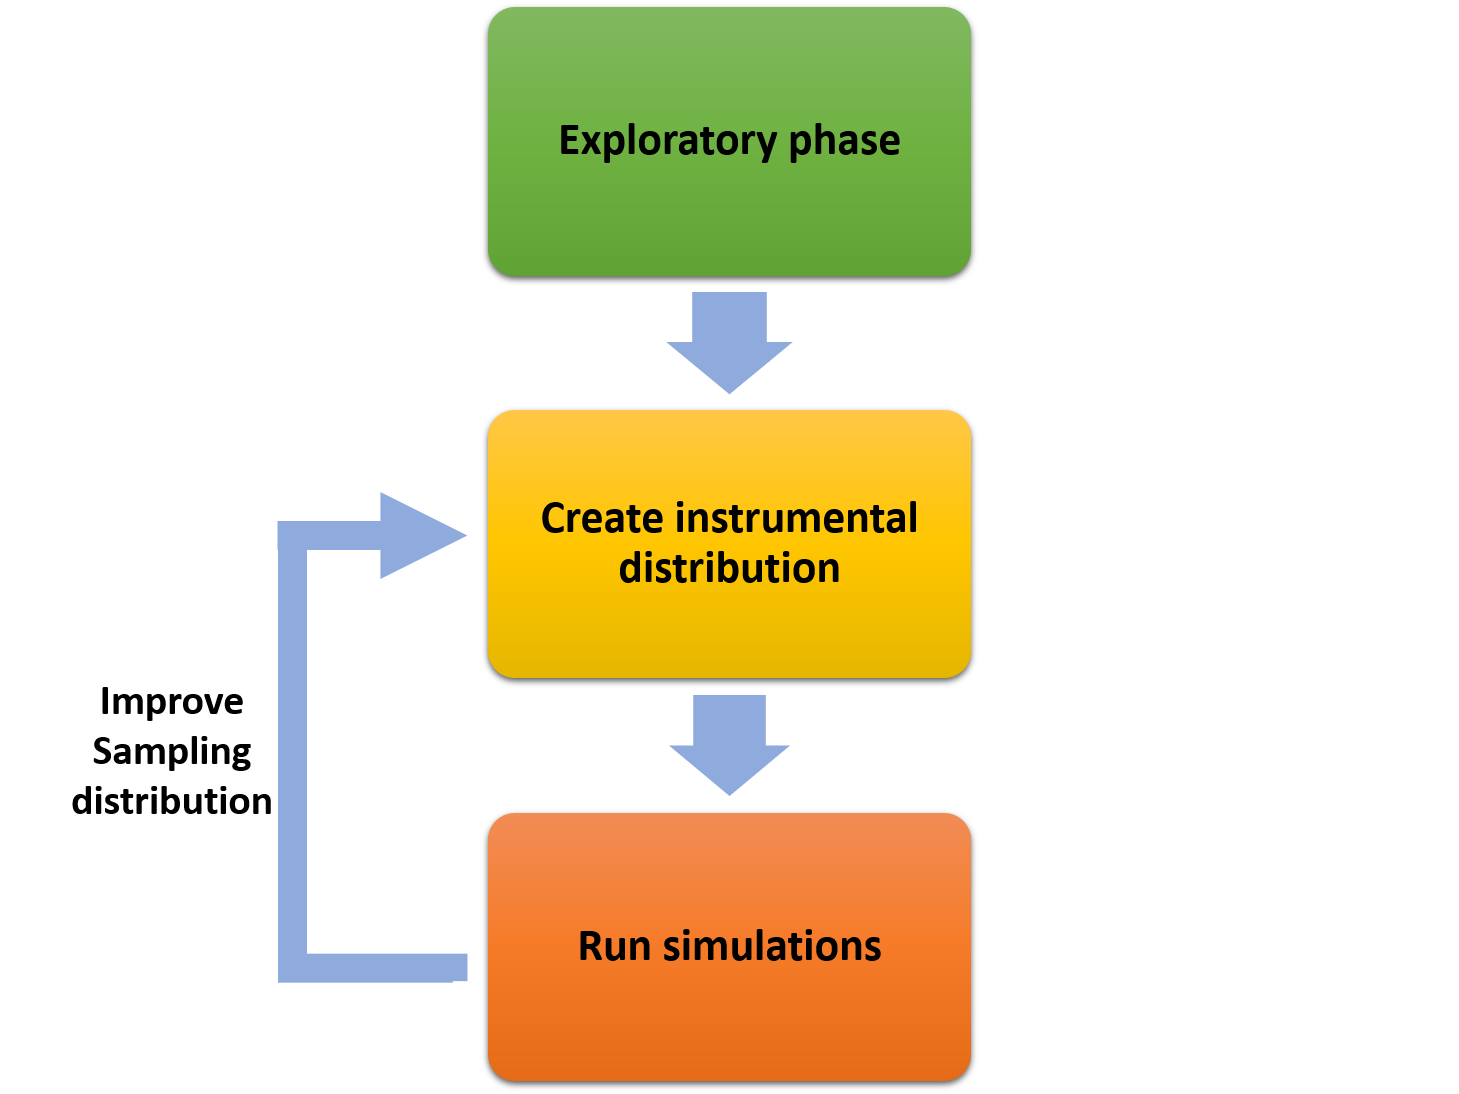
\includegraphics[width=\columnwidth]{flowchartAISv2.png}
    \caption{Flowchart of the adaptive importance sampling method that is used in this paper.  \textbf{should I add an input arrow with input priors and parameters and an output arrow for `inference'??}}
    \label{fig:aIS_scheme}
\end{figure}
%


%
%
%\subsection{Monte Carlo sampling}
%\label{subsec:MCsampling}
%%
%In monte carlo random sampling
%%
%
%
%\subsection{Uniform grid sampling}
%\label{subsec:UNIsampling}
%%
%In uniform grid
%%

\subsection{IIIb: Adaptive importance sampling Algorithm}
\label{subsec:AISalgorithm}
%
\floor{However, for our method we focus on the initial three $ M_{1,i}, a_i, q_i$. }
Assuming the parameters $M_{1,i}, q_i, a_i$ to be independent the combined prior distribution of $\mathbf{x_i}$ then becomes:
%
\begin{equation}
	p(\mathbf{x_i}) = p({M_{1,i}}) \ p({a_i}) \  p({q_i})  .
	\label{eq:prior-3d}
\end{equation} 



Since the details of binary evolution are uncertain, a large number of binaries is simulated with BPS models to thoroughly explore the space of initial conditions. The uncertainties are then captured in tunable parameters $\mathbf{x}$  which distribution functions are observably derived. Often between 3 and 20 parameters are used in BPS but for the purpose of this paper we will focus on the three most important variables: the initial mass of the primary star (i.e., the most massive star) $M_{1,i}$, the mass ratio, $q_i = M_{1,i} / M_{2,i}$, between the two stars and  the initial separation, $a_i$. Each initial binary sample can thus be represented by three parameter values
%
\begin{equation}
	\mathbf{x_i} = (M_{1,i},\ a_i, \ q_i). 
\end{equation}
%
The reason that we focus on these three parameters is (i) because above parameters are the most important  parameters in the sense that they dominate the outcome and thereby the uncertainty of the evolution (ref Belczynski $\&$ Selma or Moe?) , and (ii) that especially the primary mass and separation have an extremely steep distribution function which can drastically increase the computational costs when simulating rare events (see Section \ref{sec:aplication-I}).  The distribution functions used in this paper for the three parameters are given below. 
Although only a subsection of three parameters are used in this work,   the adaptive importance sampling method can straightforwardly be extended to all initial parameters. \\

HHHHHHHHH \\

\subsubsection{1: exploratory phase}
In step 1 of the AIS method, i.e. the Exploratory-phase,  we run COMPAS using sampling birth distribution Monte Carlo (i.e. from the standard sampling functions) until we have found a certain fixed number, N,  hits. The default of N = 100

The general idea of the AIS exploratory phase is the following: 
\begin{algorithm}
    \SetKwInOut{Input}{Input}
    \SetKwInOut{Output}{Output}

%    \underline{Exploratory phase} $(N_{\text{hits}},N_{\text{max}})$\;
%    \Input{Two nonnegative integers $N_{\text{hits}}$ and $N_{\text{max}}$}
%    \Output{$\gcd(a,b)$}
    $i = 0 $ \;
    counthits $ = 0$ \;
    \While{ \text{counthits} $\neq N_{\text{E, hits}}$  or $i \leq N_{\text{E,max}}$ }
      {
		$i += 1$        \; 
        draw new sample $x_i$\;
        evaluate sample $x_f = u(x_i)$ \;
        \If{$x_f \in X_T$}{
        counthits $+=1$ \;
        } 
      }
    \caption{Exploratory phase Algorithm}
\end{algorithm}

%
%The adaptive importance sampling (AIS) method consists of three main steps which are schematically shown in Fig. \ref{fig:aIS_scheme}. 
%\begin{enumerate}
%	\item First, there is a so-called  \emph{exploratory phase}     since it is not known a priori which part of the parameter space produces binaries of the type that is contained in the target distribution. In this phase initial samples are drawn from their birth distribution  either randomly or by creating a regular grid (uniform method) and evaluated in the model until a certain number $N_{\text{E,t}}$  of  binaries of the target type $\mathbf{X_t}$ are found. I.e. the sampling continues until  there is a set of $N_{\text{E,t}}$ binaries of the target simulation $\mathbf{x_f} \in  \mathbf{X_t}$. The choice of $N_{\text{E,t}}$ depends mostly on the aimed sampling uncertainty of the simulation and is explained further in Section \ref{subsec:standard-AIS}. 
%	\item Secondly, a new sampling distribution, $g(\mathbf{x}) $, the so-called \emph{instrumental distribution} is defined by drawing Gaussian distributions in the initial parameter space around each of the $N_{\text{E,t}}$ `successful' binaries $x_{E,k} $ with $k = 1, ..., N_{\text{E,t}}$ that evaluated to a binary system of the target population.  The instrumental distribution $g(\mathbf{x})$ is thus given by the Gaussian mixture distribution:
%	%
%	\begin{equation}
%	    g(\mathbf{x}) = \sum _{k=1}^{N_{\text{E,t}}}  g_k(\mathbf{x}) w_k =   \sum _{k=1}^{N_{\text{E,t}}}  \mathcal{N}({\boldsymbol {\mathbf{x_{t,k}},\Sigma_{k}}}) w_k 
%	\label{eq:instrumental-distribution}
%	\end{equation}	 
%	%	
%	where each $\mathcal{N}({\boldsymbol {\mathbf{x_{t,k}},\Sigma _{k}}})$ is a multivariate Gaussian distribution with mean $\mathbf{x_{E,k}}$ and covariance matrix $\mathbf{\Sigma _{k}}$. Furthermore, $w_k$ are the weights of each Gaussian distribution, which equals the weight of drawing the initial sample $x_i$ ($w_k = 1$ in the Monte Carlo random drawing). 
%	
%	\item Thirdly, new samples are now drawn from the instrumental distribution $g(\mathbf{x}) $ and evaluated with the BPS model.  Assuming the  outcome function $\phi(\mathbf{x_i})$ to be locally continuous (and not chaotic), a larger fraction of the samples will now produce binaries of the target distribution, and as a result, the simulation will model the target distribution more efficient. 
%\end{enumerate}
%After a certain number of draws, step (ii) and step (iii) can be repeated to even more increase the efficiency. 




\subsubsection{Standard implementation}

At the end of a run, the statistics of the target distribution such as the expectation value of $\phi(x)$, i.e. its rate,  and  distribution functions can be determined by using the AIS estimator

\begin{equation}
	\widetilde{\mathbb{E}[\phi(\mathbf{x})]}_{N_t} = \frac{1}{N_t} \sum_{i=1}^{N_t} \phi(\mathbf{x_i}) \frac{p(\mathbf{x_i})}{g(\mathbf{x_i})}, 
	\label{eq:ISestimator}
\end{equation}
where $N_t$ is the total number of sample drawn from the instrumental distribution. \textbf{change this to multiple generations see notes other notebook}

In general, the AIS method is based on easy to implement steps. However, many choices on for example the covariance matrices, the exploratory sampling and other sampling strategies can be made to optimize the AIS method. Below we will therefore first introduce our \emph{`standard'} AIS method which is a minimal working implementation of the AIS method that is used throughout the paper and demonstrated in section \ref{sec:aplication-I} to already reduce the simulation costs. Of course many more adjustments can be made, some of which are discussed in Subsection \ref{subsec:var_standardAIS}.     



In this subsection we will describe our so-called \emph{standard implementation} of AIS, which is used mostly throughout this paper. Although variations on this standard implementation might make the AIS method more efficient, we choose to first demonstrate the results with this more basic implementation of AIS to make it easier to understand the method and its strengths. Moreover, the choice of variations often varies for each simulation. A few examples of possible variations are discussed in the next section. 

\begin{enumerate}
	\item We choose $ N_{\text{E,t}} = 100 $ and an exploratory sampling using random draws from the birth distribution (Eq. \ref{eq:prior-3d}), i.e. Monte Carlo sampling.  We make this choice since Monte Carlo sampling produces samples with weights equal to unity, which  is the simplest sampling method for the exploratory phase of AIS. The choice of $ N_{\text{E,t}} = 100 $ implies that we will continue sampling random draws from the birth distribution until we have simulated $100$ initial binaries that evolved successfully to a target binary ($\mathbf{x_f} \in \mathbf{X_t}$). Since all samples have equal weight this implies that if we missed in our exploratory phase an area of the parameter space that also produces binaries of our target binary type, that this `missed island' most likely contributes less than $1/100$ to the total integral and thus statistics (such as the BBH fraction and/or the BBH merger rate ). 
	
	\item The instrumental distribution. Since we use random draws the weights $w_k$ in Eq. (\ref{eq:instrumental-distribution}) are equal to $ 1 / N_{\text{E,t}} $ and each Gaussian distribution contributes equally to the instrumental distribution. 
For simplicity, we  adopt a diagonal covariance matrix for $\Sigma$. Moreover, we scale the covariance matrix $\Sigma_k$  with the average expected distance locally between our initial sample points $ \mathbf{x_i}$ in the initial binary parameter space. This is chosen such that samples drawn from a Gaussian $\mathcal{N}({\boldsymbol {\mu _{i},\Sigma _{i}}})$  will generally fall in the space between the successful point  $x_i$ and its nearest neighbours.  Since the exploratory phase does not place the samples uniformly throughout the initial parameter space, e.g., many more binaries are created with low initial primary mass $M_{1,i}$ since low mass stars are much more common ( see  Eq. \ref{eq:prior-IMF}).
Therefore, we first transform the samples to a uniform sampled space, and then draw Gaussians around the space where it is uniform. This implies that the covariance matrix for the Gaussian distribution is given by

%
\begin{equation}
\Sigma_k = \begin{bmatrix} 
    \sigma_{1}^2 & 0 & \dots \\
    \vdots & \ddots & \\
    0 &        & \sigma_{d}^2 
    \end{bmatrix}, 
	\label{eq:covariance-matrix}
\end{equation}
%
where each $\sigma_{j,k} $  is given by
%
\begin{equation}
	\sigma_{j,k} =  \frac{\|p_j(x_{k, \text{max}})^{-1} - p_j(x_{k, \text{min}})^{-1} \|}{(N_{\text{E}})^{1/d}} \\
	  \text{ for } j = 1,.. ,\text{d}, k = 1, ... , N_{\text{E,t}} 
	\label{eq:sigma-covariance-matrix}
\end{equation}
%
where $p_j^{-1}$ is the inverse of the probability distribution function of the $j$-th parameter (see Subsection \ref{subsec:priorsCOMPAS}) and $N_E$ is the total number of simulations run for during the exploratory phase. 

	\item  \emph{Stopping criteria}. For the stopping criteria of the simulation we use for the standard AIS implementation to stop when a total number of $N_{\text{tot}} = XX $ samples have been evaluated. This represents the finite computational time that is often available for simulations due to scarce computational resources. Another possible stopping criteria could be defined by reaching a certain accuracy, this is further discussed in Subsection \ref{subsec:var_standardAIS}. 
	
\end{enumerate}

%\label{subsec:standard-AIS}
%\begin{itemize}
%	\item Exploratory sample
%	\item Refined sampling 
%	\item Estimators 
%	\item Stopping criteria := aimed accuracy (...) Performing inference on a finite number of simulations run induces an sampling error, this sampling error can be estimated    
%\end{itemize}
%


\subsubsection{Variations on the standard implementation}
\label{subsec:var_standardAIS}
\begin{itemize}
	\item multiple generations of $g$
	\item other ways of running exploratory run 
	\item fixed error
	\item stratified sampling 
	
\end{itemize}
%



\subsection{IIIc: Uncertainty estimates}

\subsection{IIId: Toy Model results}
See Fig. \ref{fig:ToyModel-speedUp}. 

\begin{figure}
	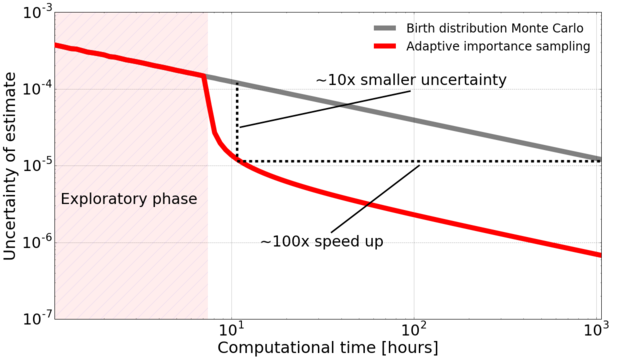
\includegraphics[width=\columnwidth]{images/speedUpToyModel.png}
    \caption{Example of   samples that are drawn (left)  uniformly distributed over the initial parameter space and (right) follow their birth distribution. The samples in the right plot are centred in the left corner since in the primary mass birth distribution used here low mass stars are much more common that high mass stars. }
    \label{fig:ToyModel-speedUp}
\end{figure}



%%%%%%%%%%%%%%%%%%%%
%%%%%%%%%%%%%%%%%%%%%


\section{4: Result I: Verification of method}
\label{sec:Verification}



\subsection{More mergers in simulation}
\label{subsec:AISsampling}
%
%
\begin{itemize}
\item 
\end{itemize}
%
See Fig \ref{fig:Progenitors_ALL}. 
The first plot is simulations from using AIS, second is from using birth distribution Monte Carlo (standard method) At first look, the speed up is factor $\sim$ 16, which is relatively low compared to the speed up I obtained with BHNSs.  I think this lower speed up is mostly due to (i) BBHs being less rare (hence bdMC is relatively better already) and (ii) for this simulation I sampled $M_1 \in [8,100]$ which also helps. But I will probably change this (for consistency) to $[5,100]$  as Simon and Alejandro suggested.


Btw, besides the speed up, Im actually most excited for the fact that in the AIS plot we find some islands  that we didnt find with bdMC. With this I mean that at least in these two simulations AIS finds a bigger variety of progenitors than MC. This is visible e.g. when you look at the hits for GW170814 where AIS finds (more) events with $q_BH$ $\sim$ 1. But e.g. also for LVT151012 where in the AIS more extreme $q_BH$ sources are found for LVT151012. (But of course this can still be ``just luck``)

But I'm excited since at least so far it doesn't look like we are missing small islands when running AIS compared with bdMC (which was/is my major concern)


\begin{figure*}
	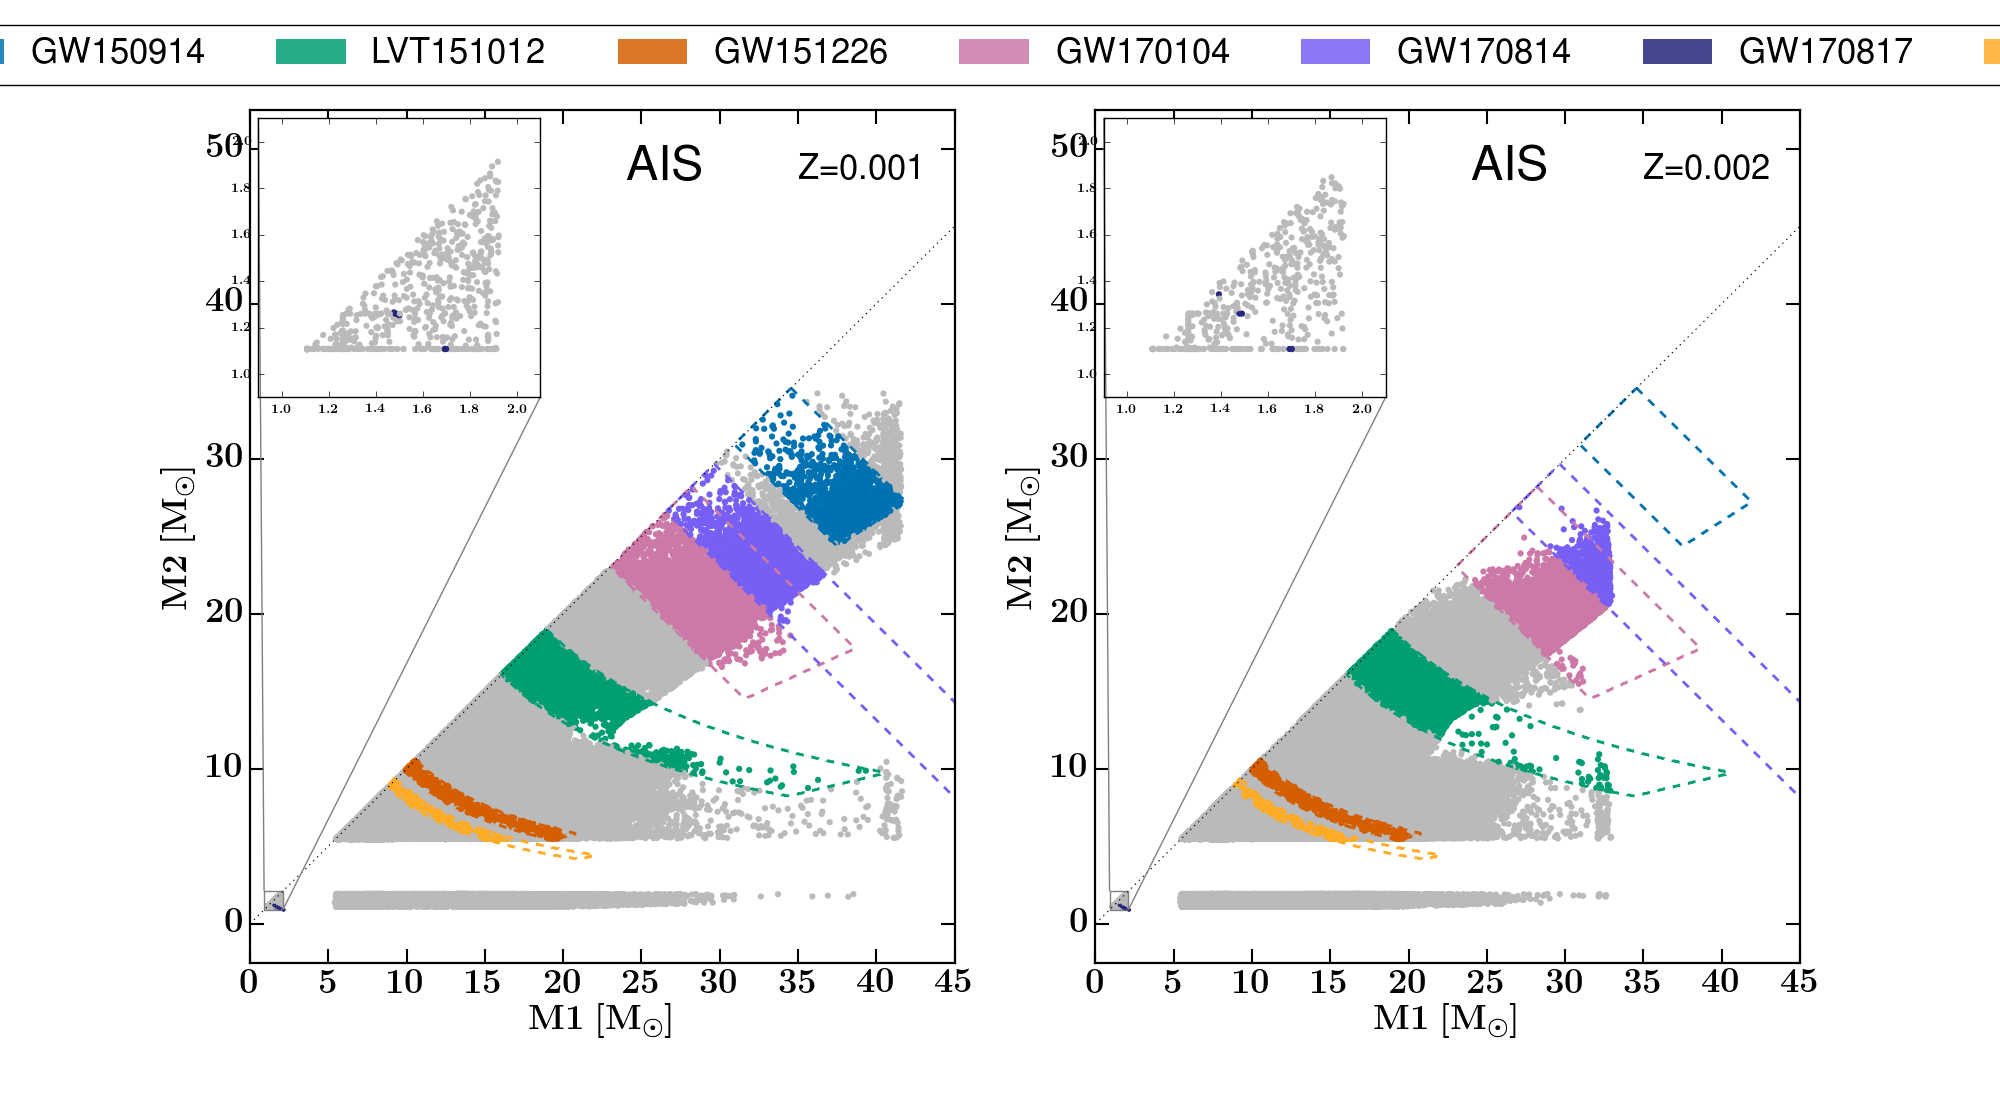
\includegraphics[width=0.8\textwidth]{images/M1M2DCOsAIS.png}
    \caption{ \floor{WILL BE FIGURE SHOWING INCREASE OF SAMPLES FOR ALL MERGERS MC vs AIS}. Example of   samples that are drawn (left)  uniformly distributed over the initial parameter space and (right) follow their birth distribution. The samples in the right plot are centred in the left corner since in the primary mass birth distribution used here low mass stars are much more common that high mass stars. }
    \label{fig:Progenitors_ALL}
\end{figure*}
\begin{figure*}
	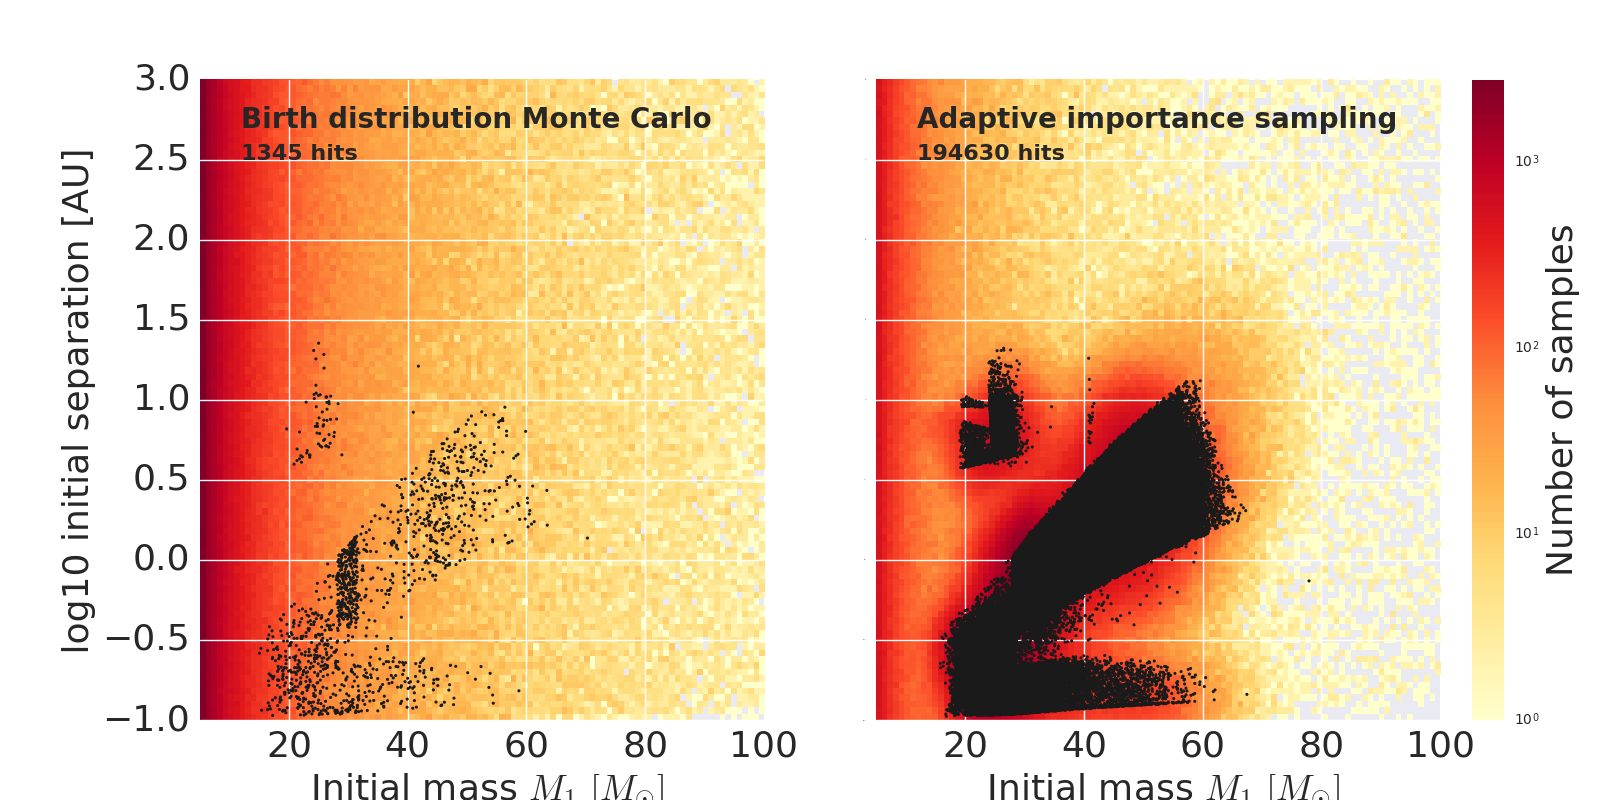
\includegraphics[width=0.8\textwidth]{images/BHNScomparisonM1ZAMSseparationInitialFixedCPUtime.png}
    \caption{\floor{WILL BE FIGURE SHOWING INCREASE OF SAMPLES FOR BH-NS MERGERS MC vs AIS. }}
    \label{fig:Progenitors_BHNS}
\end{figure*}


\subsection{ Rate estimator / speed ups}
\label{subsec:RateI}
%%\newcommand\SpeedUpBHNStwo{16}
%\newcommand\SpeedUpBHNStwoTenmillion{80}
%\newcommand\HitsBHNSMCtwo{1345}
%\newcommand\HitsBHNSAIStwo{179392}
%\newcommand\fractionMoreHitsBHNStwo{133}
%Range $M_1$ &
\begin{table*} %{Summary of Adaptive Importance Sampling method results \\}
\centering
\label{my-label}
\begin{tabular}{|l|l|l|l|l|l|l|l|l|}
\hline
Target subpopulation        & Metallicity & $N_{\text{hits,MC}}$ & $ N_{\text{hits,AIS}}$ & $F_{\text{more hits}}$ 		 &  $\rate_{\text{MC}}$  & $\rate_{\text{AIS}}$   & S$_{10^6}$         & S$_{10^7}$  					\\
						    &			  &	 		 			 & 	 					  &	           		  		& [year]      & [year]       & 	&  	\\ \hline
ALL mergers in $\tau_{H}$   & Z = 0.001    & \HitsALLMCone 		 & \HitsALLAISone 		  & \fractionMoreHitsALLone &  		   &  			  & \SpeedUpALLone  & \SpeedUpALLoneTenmillion \\
						    & Z = 0.002   & \HitsALLMCtwo 		 & \HitsALLAIStwo 		  & \fractionMoreHitsALLtwo &  		   &  			  & \SpeedUpALLtwo  & \SpeedUpALLtwoTenmillion \\
BH-BH mergers in $\tau_{H}$ & Z = 0.001   &  & & & &  &  &  \\ %\hline
						    & Z = 0.002   &  & & & &  &  &  \\ %\hline
NS-NS mergers 				& Z = 0.001   &  & & & &  &  &  \\ %\hline
						    & Z = 0.002   &  & & & &  &  &  \\ %\hline
BH-NS mergers in $\tau_{H}$ & Z = 0.001   & \HitsBHNSMCone 		 & \HitsBHNSAISone 		  & \fractionMoreHitsBHNSone &  		   &  			  & \SpeedUpBHNSone  & \SpeedUpBHNSoneTenmillion \\ 
						    & Z = 0.002   & \HitsBHNSMCtwo 		 & \HitsBHNSAIStwo 		  & \fractionMoreHitsBHNStwo &  		   &  			  & \SpeedUpBHNStwo  & \SpeedUpBHNStwoTenmillion \\ %\hline
						    &  &  &  &  & & & &  \\ %\hline
						    &  &  &  &  & & & &  \\ \hline
%\begin{tabular}{|l|l|l|l|l|l|l|l|}
%\hline
%Target subpopulation           			  & Metallicity &  $ N_{\text{hits, AIS}}/ N_{\text{hits, bdMC}}$ &  &  $\rate$ MC & $\rate$  AIS & Speed up  & \\
%										  & 			& [	$ M_{\odot}$] 		   & 						&			  & 			[year] 	& [year] &  & \\ \hline
%All DCO mergers in $\tau_{\text{Hubble}}$ & $Z = 0.001$             &                         &                        &                 &    &          &  \\ \hline
%                               & $Z = 0.002$           &                         &                        &                  &                   &    &      \\ \hline
%BBH mergers in Hubble time     & Z = 0.001                            &                         &                        &                  &                   &        &  \\ \hline
%                               & Z = 0.002                            &                         &                        &                  &                   &       &   \\ \hline
%BNS mergers                    & $Z = 0.001$                          &                         &                        &                  &                   &      &    \\ \hline
%BNS mergers                    &  $Z = 0.002$                         &                         &                        &                  &                   &       &   \\ \hline
%BH-NS mergers                  & Z = 0.001                &                         &                        &                  &                   & 100      \\ \hline
%BH-NS mergers                  & Z = 0.002                            &                         &                        &                  &                   & 100    &  \\ \hline
%                               &                                      &                         &                        &                  &                   &      &    \\ \hline
\end{tabular}
\caption{Summary of the results of comparing simulations run with our Adaptive Importance Sampling (AIS) sampling method, and a simulation run with traditional Monte Carlo (bdMC) sampling, where binaries are drawn from their birth distributions. In both cases we use our \Fiducial model.  We compare the results for different examples of target populations of binaries.  $N_{\text{hits,bdMC}}$ and $N_{\text{hits,AIS}}$ are the number of binaries (i.e. `hits') found  when running the simulation with bdMC and AIS respectively. $ F_{\text{more hits }}$ is the factor of more hits that we found when using AIS over bdMC for a simulation with $10^6$ binaries for bdMC  ($\sim 170$ CPU hours)  $ F_{\text{more hits }} = N_{\text{hits,AIS}}/ N_{\text{hits,bdMC}}$. $\rate_{\text{MC}}$  and $\rate_{\text{AIS}}$ are the rates computed with bdMC and AIS respectively. S$_{10^6}$ and S$_{10^7}$ are the computational speed ups of the simulation when comparing with a bdMC run of respectively $10^6$ and $10^7$ binaries. }
\end{table*}


%
\begin{itemize}
\item 
\end{itemize}
%


\section{Black Hole - Neutron Star simulations}
\label{sec:BHNSresults}
\subsection{Better (Chirp mass) distribution}
\label{subsec:ChirpDistributionI}
%
\begin{figure}[h]
	%\myfloatalign
	{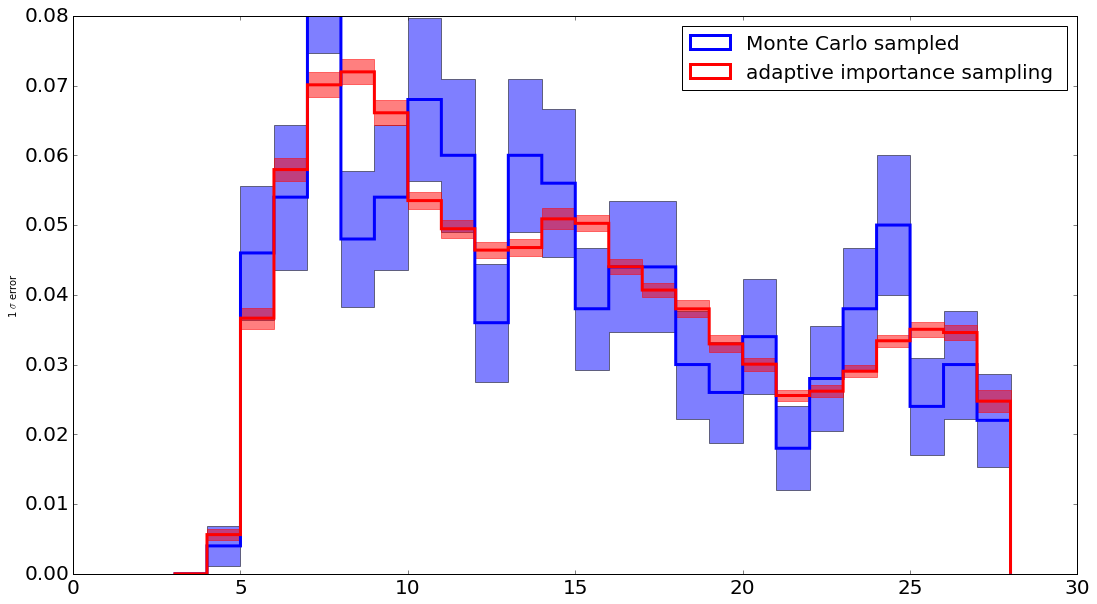
\includegraphics[width=1\linewidth]{images/histogram_2}}
\caption{}\label{fig:ToyModel-snakeplot}
\end{figure}

\subsection{better subchannels}
\begin{figure}[h]
	%\myfloatalign
	{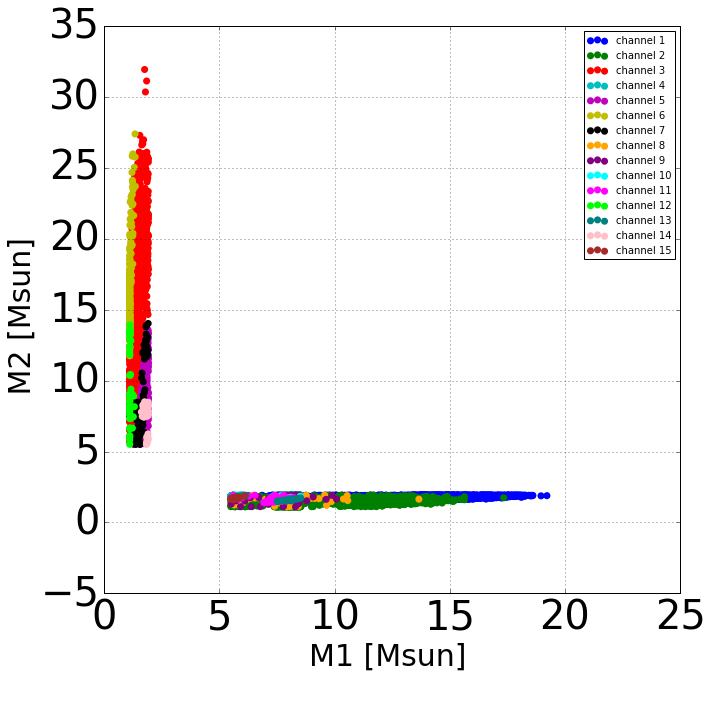
\includegraphics[width=1\linewidth]{images/Channalsv0}}
\caption{}\label{fig:BHNS-subchannels}
\end{figure}

\subsection{Covering more rare events}

FOR EXAMPLE HIGH KICKS!


\subsection{smaller uncertainties on rates}




%
\begin{itemize}
\item 
\end{itemize}
%



\section{Astrophysics BH-NSs and variations}
\label{sec:variationsBHNS}




\subsection{explain subchannels}


\subsection{Rates?}

\subsection{Variations}
\begin{table*}
\caption{
We list all simulations computed for this study; for simulations 02 through 19, we state the physical interaction or assumption varied relative to the \texttt{Fidicual} model and the actual parameter varied.
For each simulation, we give the formation rate $\rate$ of DNS which will merge in a Hubble time in the Galaxy and its log Bayes factor relative to the \texttt{Fidicual} model model (see Appendix \ref{sec:likelihood}) given the observed Galactic DNS period-eccentricity distribution.
See figure \ref{fig:nineteenpanels} for the predicted period--eccentricity distributions for all models.
}
\label{tab:models}
\begin{tabular}{lccccc}
\hline
Number & Physics & Variation  & $\rate$~[\textrm{$\rm Myr^{-1}$}]	& $\textrm{log}(\mathcal{K})$ \\
\hline
%00 & \texttt{$\rm COMPAS\_\alpha$} & & \formationVarZero & \bayesVarZero\\
01 & $\rm COMPAS$ \texttt{Fiducial} & &  &  \\
02 & Stability & Case BB: unstable &  &  \\
03 & SNe & Fryer Delayed &  &  \\
04 & SNe & M\"uller &&  \\
05 & SNe & Single Mode & & \\
06 & SNe & $\sigma_{\textrm{ECSN}}=\sigma_{\textrm{high}}$  & & \\
07 & SNe & $\sigma_{\textrm{USSN}}=\sigma_{\textrm{high}}$  & & \\
08 & CE & $\lambda=0.1$  & & \\
09 & CE & $\lambda_{\textrm{Kruckow}}\propto R^{-5/6}$  & & \\
10 & CE & $\alpha=0.1$  & & \\
11 & CE & $\alpha=10.0$  & & \\
12 & Circularisation & $a_{\rm p}=a(1-e)$  & & \\
13 & Circularisation & $a_{\rm SR}=a(1-e^2)$  & &\\
14 & Mass Loss Mode & Jeans  & & \\
15 & Mass Loss Mode & Circumbinary  & & \\
16 & Distribution & $f_{e}(e)=$ Thermal  & & \\
17 & Metallicity & Z=0.002  & & \\
18 & Metallicity & Z=0.001 & & \\
19 & CE & Pessimistic  & & \\
\hline
\end{tabular}
\end{table*}
\subsubsection{SN mechanism}
As a variation we also explore the `delayed' scenario from \citep{fryer2012compact}.

\subsubsection{metallicities}

\subsubsection{eccentricity}

\subsubsection{higher subkick}
To explore variations on this model we also simulate a population of black hole-neutron stars with a singe mode kick distribution, and with different peak values for the low-mass iron (or oxygen-neon-magnesium) cores kick. \floor{explain and read more about USN ECN etc. and prescription in COMPAS}.
\subsubsection{different kick distribution}

\subsubsection{PISN Belczynski}



%\section{Application II}
%\label{sec:aplication-II}
%%
%\begin{itemize}
%\item 
%\end{itemize}
%%



\section{Discussion}
\label{sec:discussion}
%
\begin{itemize}
\item caveat: physics BPS not brilliant
\item Expl can be better
\item More adaptive
\item more parameters
\item 
\end{itemize}
%

\section{Summary }






\section*{Acknowledgements}

We thank the the Kavli Foundation, Niels Bohr institute and DARK Cosmology Centre in Copenhagen for their hospitality and for organising the Kavli summer school in gravitational waves astrophysics 2017. This work could not have been done without their support. 

%%%%%%%%%%%%%%%%%%%%%%%%%%%%%%%%%%%%%%%%%%%%%%%%%%

%%%%%%%%%%%%%%%%%%%% REFERENCES %%%%%%%%%%%%%%%%%%

% The best way to enter references is to use BibTeX:
\newpage 

\bibliographystyle{mnras}
\bibliography{my_bib} % if your bibtex file is called example.bib


% Alternatively you could enter them by hand, like this:
% This method is tedious and prone to error if you have lots of references
%\begin{thebibliography}{99}
%\bibitem[\protect\citeauthoryear{Author}{2012}]{Author2012}
%Author A.~N., 2013, Journal of Improbable Astronomy, 1, 1
%\bibitem[\protect\citeauthoryear{Others}{2013}]{Others2013}
%Others S., 2012, Journal of Interesting Stuff, 17, 198
%\end{thebibliography}

%%%%%%%%%%%%%%%%%%%%%%%%%%%%%%%%%%%%%%%%%%%%%%%%%%

%%%%%%%%%%%%%%%%% APPENDICES %%%%%%%%%%%%%%%%%%%%%

\appendix





\section{ToyModel}


\subsection{Distribution functions}

\begin{figure}[h]
	%\myfloatalign
	{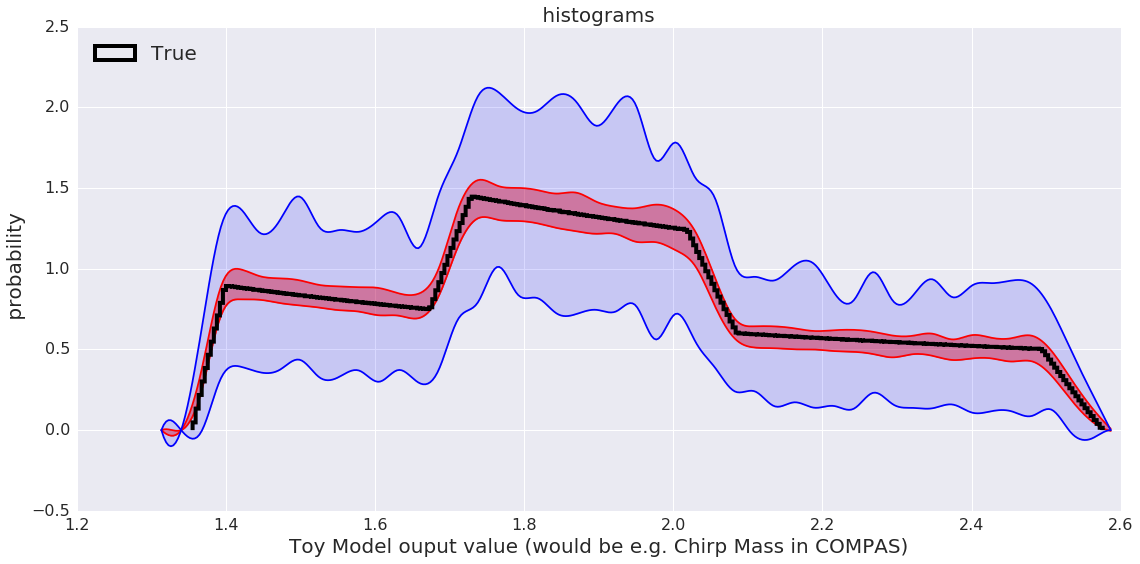
\includegraphics[width=1\linewidth]{images/snakeplot_pdff1}}
\caption{}\label{fig:ToyModel-snakeplot}
\end{figure}

I chose now two analytical output functions (one continuous $f_1$ and one discontinuous $f_2$) such that I know the " true" (i.e. analytical) distribution and cdf.
I then ran simulations using both birth distribution Monte Carlo (standard method) and AIS and compared the distributions from these simulations with the true distribution.

At this moment I quantisized the " goodness of estimates of the distributions"  by comparing KS tests.
Attached you can find a plot that shows this test.

The plots are for relatively function f1 and f2. The right panel shows the true cdf (black) in addition to the cdf from a simulation run with 100000 samples with birth distribution Monte Carlo (blue) and AIS (green). Already from the right panel you can clearly see that the AIS cdf lies much closer to the true cdf.
However, note that the results of course are also still random, so the right panel is just capturing one simulation and thus " one estimate of the cdf"

So next, I rerun the simulation 100 times (in other words I would get 100 AIS- and 100 birth distribution Monte Carlo cdfs), and for each simulated cdf I calculated the KS-statistic, which is a measure for how close the simulated cdf lies to the true cdf.

So in the end, for both the AIS and birth distribution I end up with a distribution of KS-statistic values, which are plotted in a violin plot in the left panel.
The width of these violins don't really matter, but what you could notice in these plots is that
(i) the green violin (AIS) lies lower than the blue violin (birth distr MC), i.e. the KS-statistics for AIS simulations lie closer to 0, which means they are closer to the true cdf.
(ii) the height of the AIS violin is smaller than the birth distr MC violin, which means the KS-statistics have smaller variance, and thus the cdf differ less from each other.

I'm still thinking about other ways to quantify how good a distribution is resolved. Maybe by comparing p-values or doing Bayesian,..






$\rightarrow$
 I will definitely make a plot that shows the KS-statistics as a function of increasing computational costs (and 1sigma interval) 
\begin{figure}[h]
	%\myfloatalign
	{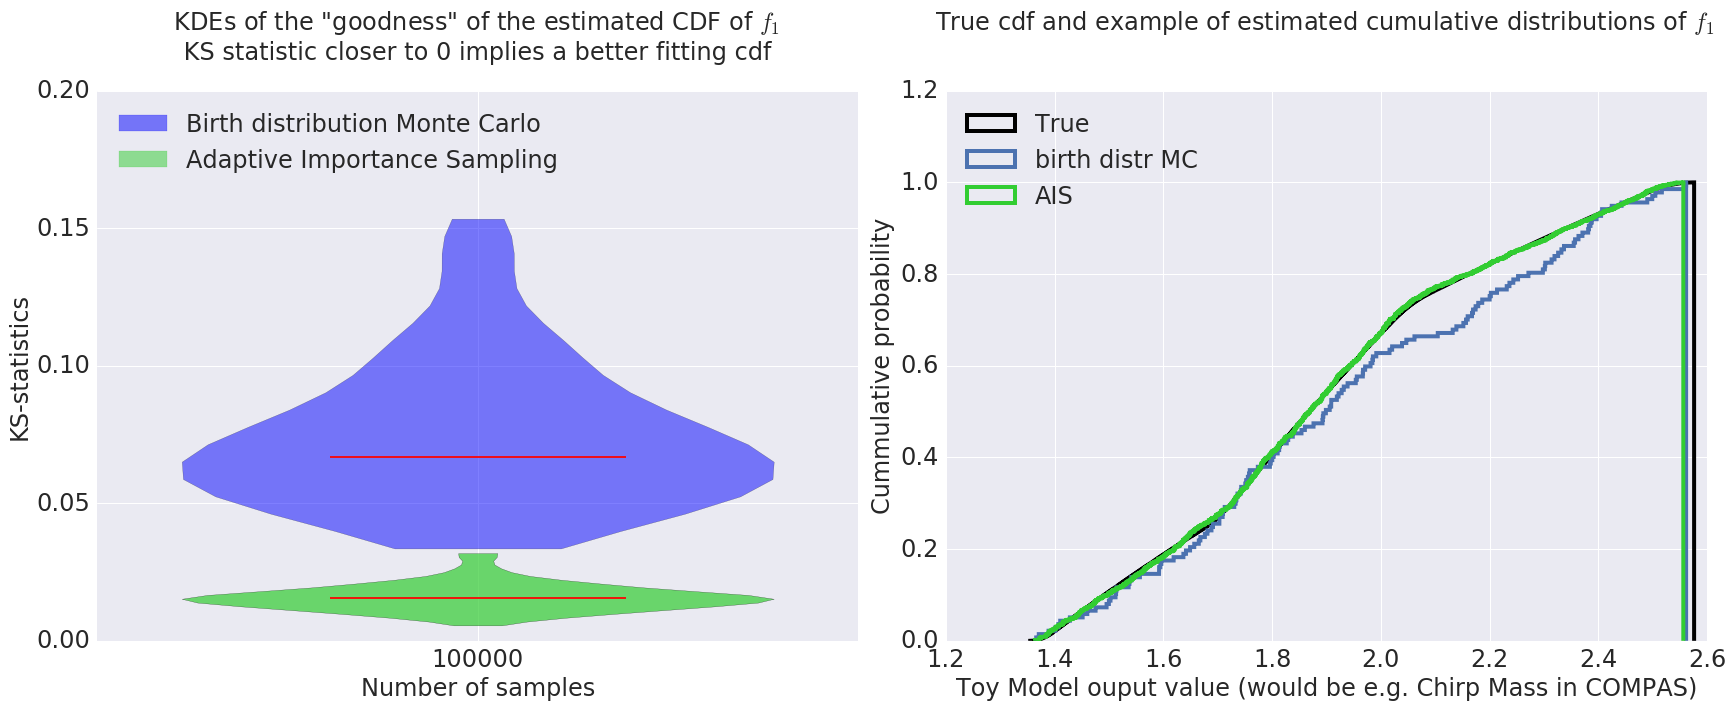
\includegraphics[width=1\linewidth]{images/CDF_KStest_combined_f1}}
\caption{}\label{fig:ToyModel-KStests}
\end{figure}


\begin{figure}[h]
	%\myfloatalign
	{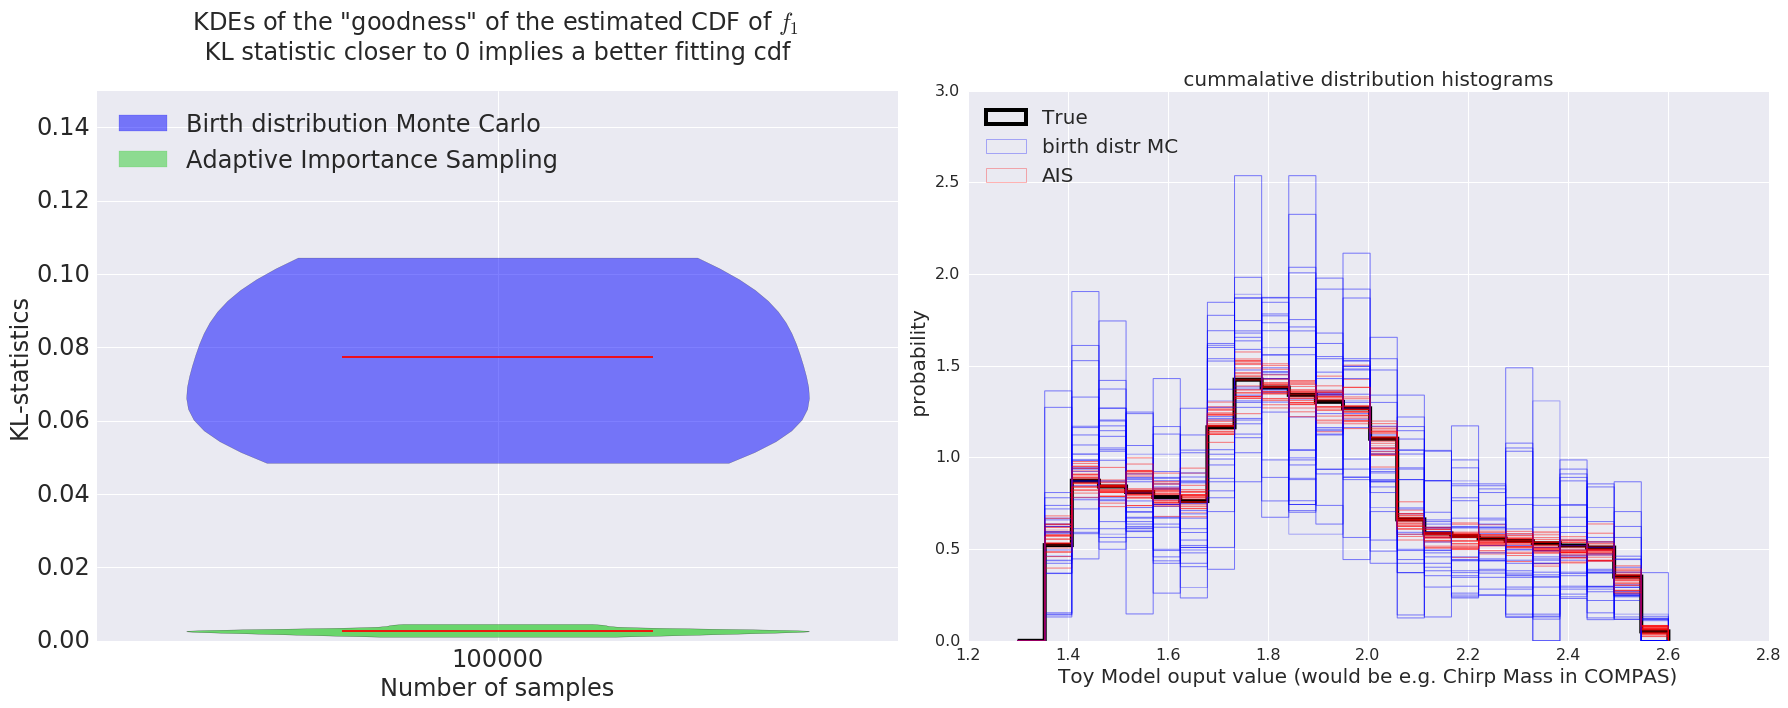
\includegraphics[width=1\linewidth]{images/Combined_KLviolin_andPDFs-toymodel}}
\caption{}\label{fig:ToyModel-KLtests}
\end{figure}



\subsection{Rates}

\begin{figure}[h]
	%\myfloatalign
	{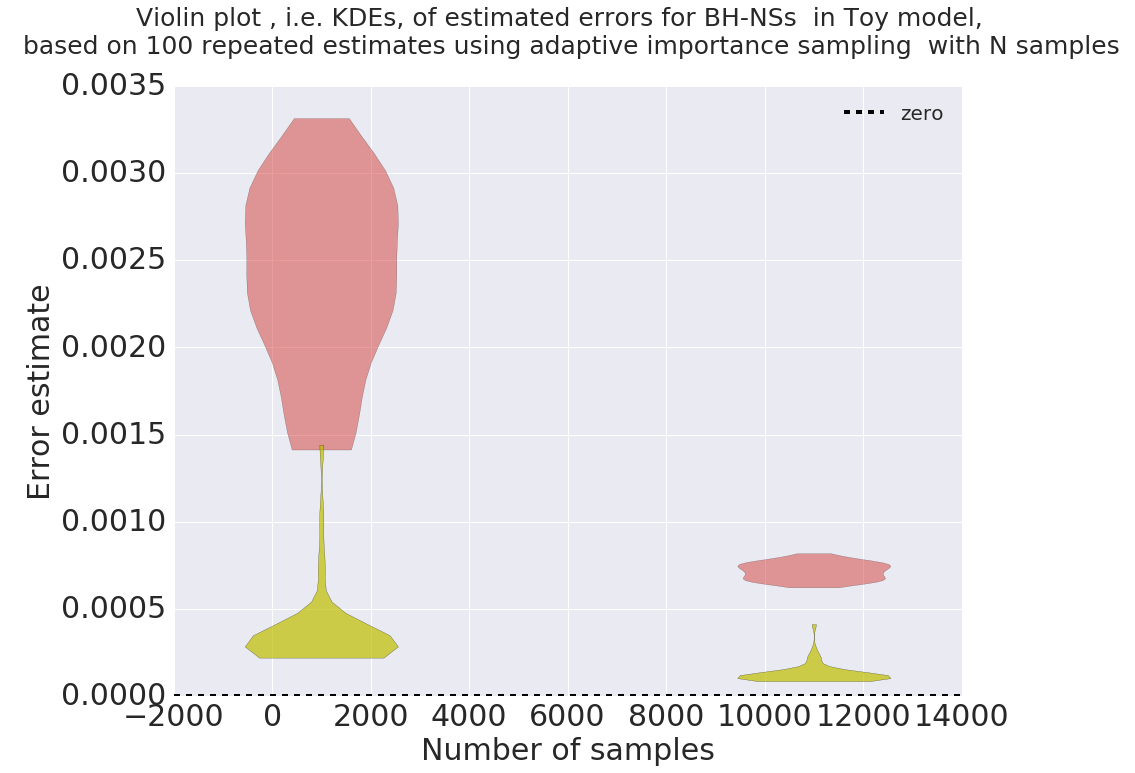
\includegraphics[width=1\linewidth]{images/ViolinErrorsCombined}}
\caption{}\label{fig:ToyModel-ViolinErrorsCombined}
\end{figure}

\begin{figure}[h]
	%\myfloatalign
	{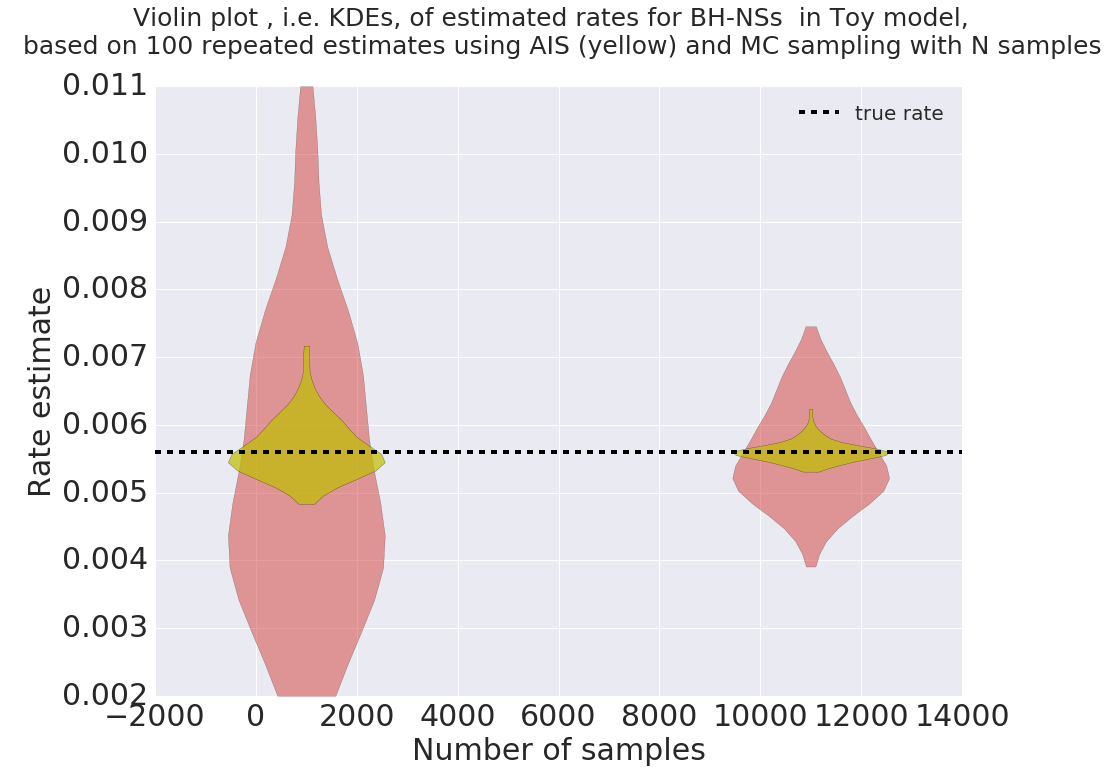
\includegraphics[width=1\linewidth]{images/ViolinvCombined}}
\caption{}\label{fig:ToyModel-ViolinvCombined}
\end{figure}




\section{Distributions}

\begin{figure*}
	%\myfloatalign
	{\includegraphics[width=0.8\textwidth]{/home/floor/Documents_Thesis/DataAnalysis/images/BHNSHistogramGrid}}
\caption{Histograms of several initial and output parameters for BH-NS mergers from simulations using Adaptive Importance Sampling (AIS) (gray) and the traditional method birth distribution Monte Carlo sampling.  Using AIS sampling, more binaries of the target distribution are found, resulting in a smoother distribution function (with smaller error bars).}\label{fig:ToyModel-ViolinErrorsCombined}
\end{figure*}


%%%%%%%%%%%%%%%%%%%%%%%%%%%%%%%%%%%%%%%%%%%%%%%%%%


% Don't change these lines
\bsp	% typesetting comment
\label{lastpage}
\end{document}

% End of mnras_template.tex
